\subsubsection{\theoryC{Precision predictions for new dilepton and $t\bar t$ resonances}}
\contributors{M. Altakach, J. Fiaschi, T.~Je\v{z}o, M. Klasen, I. Schienbein}\rt{There are comments to address.}
%{\bf Author(s): M. Altakach$^1$, J. Fiaschi$^2$, T.~Je\v{z}o$^3$, M. Klasen$^4$,
%I. Schienbein$^5$}
%
%\vspace*{1ex}
%
%\noindent
%$^1$ Laboratoire de Physique Subatomique et de Cosmologie, Universit\'e Grenoble Alpes, CNRS/IN2P3, 
%53 Avenue des Martyrs, F-38026 Grenoble, France
%\\
%altakach@lpsc.in2p3.fr
%
%\noindent
%$^2$ Institut f\"ur Theoretische Physik, Westf\"alische Wilhelms-Universit\"at M\"unster,
%Wilhelm-Klemm-Stra{\ss}e 9, D-48149 M\"unster, Germany
%\\
%fiaschi@uni-muenster.de
%
%\noindent
%$^3$ Physics Institute, Universit\"at Z\"urich, Z\"urich, Switzerland
%\\
%tomas.jezo@physik.uzh.ch
%
%\noindent
%$^4$ Institut f\"ur Theoretische Physik, Westf\"alische Wilhelms-Universit\"at M\"unster,
%Wilhelm-Klemm-Stra{\ss}e 9, D-48149 M\"unster, Germany
%\\
%michael.klasen@uni-muenster.de
%
%\noindent
%$^5$ Laboratoire de Physique Subatomique et de Cosmologie, Universit\'e Grenoble Alpes, CNRS/IN2P3, 
%53 Avenue des Martyrs, F-38026 Grenoble, France
%\\
%ingo.schienbein@lpsc.in2p3.fr

%\subsubsection{Introduction} 
%\paragraph*{Introduction} 

%\noindent 
We present higher order predictions for spin-1 resonance searches in two classes of observables,
top-quark-pair production and dilepton production.
In the former case, we use the {\tt PBZp} code~\cite{Bonciani:2015hgv} which includes the next-to-leading order (NLO)
QCD corrections to the electroweak production of top-antitop pairs in the presence of a new neutral gauge boson 
implemented in the parton shower Monte Carlo program {\tt POWHEG}~\cite{Frixione:2002ik,Frixione:2007vw,Alioli:2010xd}.
The dilepton cross sections are calculated using the NLO+NLL  code {\tt Resummino}~\cite{Jezo:2014wra} which matches
a soft-gluon resummation at next-to-leading logarithmic (NLL) accuracy to a fixed order NLO calculation.

We consider four models: the Un-Unified (UU)~\cite{Georgi:1989ic,Georgi:1989xz} and the Non-Universal (NU)~\cite{Malkawi:1996fs,Li:1981nk}
models, a leptophic topcolor model (TC) (model IV in \citeref{Harris:1999ya}), and the Sequential Standard Model (SSM)~\cite{Altarelli:1989ff}.
The UU and NU models belong to the general class of G(221)$={\rm SU}(2)_1 \times \rm{SU}(2)_2 \times U(1)_X$ gauge theories 
with an extra SU(2) gauge symmetry.
In the UU model the quarks and leptons  belong to different representations of the two SU(2) gauge factors whereas in the NU model
the first two generations transform differently than the third generation. Both models take two input parameters, the mixing angle 
of the first stage symmetry breaking  $t=\tan \phi = g_2/g_1$ and the mass of the heavy resonance $M_{Z'}$ (or $M_{W'}$).
Exclusion limits on the parameters space for the G(221) models have been derived in \citeref{Hsieh:2010zr} by performing 
a global analysis of low-energy precision data. Improved limits for the $W'$ and $Z'$ masses were found in \citeref{Jezo:2014wra} using LHC 
data at $\sqrt{s}=7$ and 8 TeV.
The TC model has three free parameters in addition to the resonance mass $M_{Z'}$: 
the width $\Gamma_{Z'}$, the relative strength ($f_1$) of the $Z'$ coupling 
to right-handed up-type quarks w.r.t. left-hand up-type quarks, and similarly the relative stregth ($f_2$) of the $Z'$ coupling to right- and left-hand down-type quarks. 
Finally, in the SSM the only free parameters are the masses $M_{W'}$ and $M_{Z'}$.

We have chosen benchmark points such that the width $\Gamma_{Z'}$ in all models is the same as in the SSM.
We have calculated the width in the SSM ($\Gamma_{Z'}^{\rm SSM}$) at leading order using PYTHIA6~\cite{Sjostrand:2014zea} with a running 
electro-magnetic coupling, $\alpha(M_{Z'})$, such that $\Gamma_{Z'}^{\rm SSM}/M_{Z'}$ slightly increases from $3.48\%$ at $M_{Z'} =1$ TeV
to $3.61\%$ at $M_{Z'} =10$ TeV.
This is achieved by setting the parameter $t=1$ in the UU and NU models. As a consequence, the $W'$ couplings to the Standard Model fermions
are the same in the SSM and NU cases, whereas the $Z'$ couplings are different.
For the TC model we set  $f_1 = 1$ and  $f_2=0$ which maximes the fraction of $Z'$ bosons decaying into $t \bar t$ pairs.
For the parton distribution functions (PDFs), in the $t \bar t$ case, we use a NLO PDF4LHC set for Monte Carlo studies (ISET = 90000 in LHAPDF6)  and the renormalisation and factorisation scales $\mu_R$ and $\mu_F$ are identified with the squared invariant mass of the system.
On the other hand, in the dilepton case, we use a NLO CT14 (ISET = 13100 in LHAPDF6) and the renormalisation and factorisation scales $\mu_R$ and $\mu_F$ are identified with the squared invariant mass of the system. \rt{why squared mass?}
%\subsubsection{Results for $t\bar t$ resonances with {\tt PBZp}}
%\paragraph*{Results for $t\bar t$ resonances with {\tt PBZp}}

In \fig{fig:POWHEG_uu_nu_tc}, we show the total cross section for the electroweak production of $t \bar t$ pairs 
($q \bar q \to Z' \to t \bar t [+g]$) in picobarn at a \com energy $\sqrt{s} = 14$ TeV (left) and $27$ TeV (right). 
The results are given for LO (only for SSM) and NLO cross sections together with the NLO/LO K-factors (bottom)
for the SSM, UU, NU, and TC in dependence of the $Z'$ mass.
No cut on the invariant mass of the $t \bar t$ pair has been applied.
\begin{figure}
\centering
{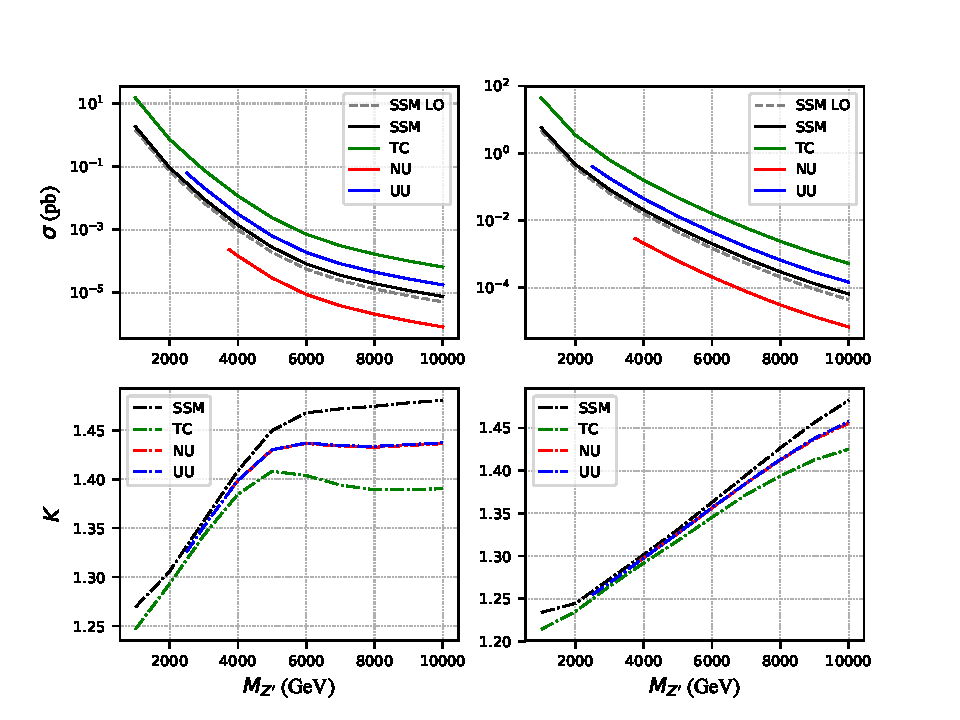
\includegraphics[scale=1]{\main/section7OtherSignatures/img/POWHEG_UU_NU_TC_14_27.pdf}}
\caption{ Left: LO and NLO total cross section predictions in picobarns for $q \bar q \to Z' \to t \bar t [+g]$ (top) 
 and the NLO/LO K-factors(bottom) at a \com energy $\sqrt{s}= 14$ TeV. Right: same as the left for a \com energy $\sqrt{s}= 27$ TeV. 
\label{fig:POWHEG_uu_nu_tc}}
\end{figure}
%\subsubsection{Results for dilepton resonances with {\tt Resummino}}
%\paragraph*{Results for dilepton resonances with {\tt Resummino}}

In \fig{fig:dilepton_ssm} we show the  $W'$ production cross sections  at a \com energy $\sqrt{s} = 14$ TeV at NLO and NLO+NLL in the SSM as a function of the heavy gauge boson mass (top left). The ratios of the total cross sections at LHC14 at NLO and NLO+NLL over the LO cross section as a function of the $W'$ mass is also presented (bottom left).
Similarly, in the right side of \fig{fig:dilepton_ssm}  we show the same for a \com energy $\sqrt{s} = 27$ TeV.
 Interference terms between $W$ and $W'$ gauge bosons are included. The
 invariant mass of the lepton pair is restricted to $m_{ll}>3M_{W'}/4$. Increasing the mass the threshold effects become more and more important leading to almost $16\%$ $(6\%)$ increase of the cross section at $M_{W'} = 8$ TeV for $\sqrt{s} = 14$ $(27)$ TeV.
 
  \begin{figure}
\centering
{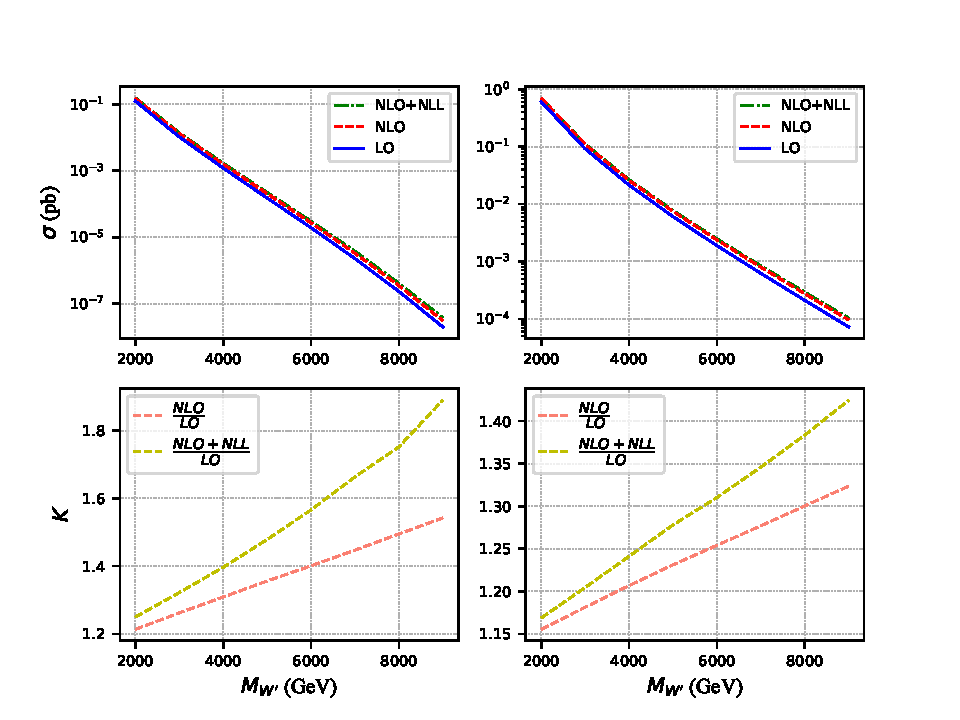
\includegraphics[scale=1]{\main/section7OtherSignatures/img/Resummino_tot_SSM_Wp_14_27_13100.pdf}}
\caption{ Left: LO, NLO, and NLO+NLL total cross section predictions in picobarn for $q \bar q \to W|W' \to e  \nu$ (top). The NLO/LO and the NLO+NLL/LO K-factors at a \com energy $\sqrt{s}= 14$ TeV (bottom). Right: same as the left for a \com energy $\sqrt{s}= 27$ TeV. 
\label{fig:dilepton_ssm}}
\end{figure}
  %\caption{NLO and NLO+NLL total cross section predictions in attobarns for %$q \bar q \to W|W' \to e  \nu$ 
 %and the NLO/LO K-factors at a \com energy $\sqrt{S}= 14$ TeV.}
% Interference terms between $W$ and $W'$ gauge bosons are included. The
% invariant mass of the lepton pair is restricted to $Q>3M_{\Wp}/4$.}
%%%%%%%%%%%%%% Start of Table  %%%%%%%%%%%%%%%%%%%%%%%%%%%%%%%%%


\paragraph*{Acknowledgements}
The work of M.K.~has been supported by the BMBF under contract 05H15PMCCA and the DFG through the Research Training Network 2149
``Strong and weak interactions - from hadrons to dark matter''.
T.J.~was supported by the Swiss National Science Foundation~(SNF) under contracts BSCGI0-157722 and CRSII2-160814.
